\documentclass[conference,compsoc]{IEEEtran}

\bibliographystyle{plain}
\usepackage[dvipdfmx]{graphicx}
\usepackage{listings,jlisting}
\usepackage{ascmac}
\usepackage{algorithm}
\usepackage{algorithmic}
\title{Extended Top Down Method from SR model to Runnables in AUTOSAR}
\author{Shunsuke Hori}

\begin{document}

\maketitle

\begin{abstract}
 Model based development has become important.
In MATLAB/Simulink which is a model based development tool, synchronous reactive models (SR models) are used.
Using SR models, developers can describe AUTOSAR software components.
Then, developers must map blocks of SR models to AUTOSAR runnables that are units of processing in AUTOSAR.
This paper proposes a top down mapping method from SR models to runnables considering optimal schedulability and modularity, while achieving schedulability and code size.
jfs
\end{abstract}
	\section{INTRODUCTION}
 Embedded system development has become large scale and complication innovation of process in embedded system development is needed.
Conventionally, we develop it with paper specification, well we would like to use tools, for example MATLAB/Simulink, to realize low-cost and fast development.
This is Model base development.
Four characteristics of Model based development is as below.
	\begin{itemize}
		\item Representation or definition of a measure due to a model
		\item Verification due to simulation from a model
		\item Automatic code generation from a model
		\item Reuse of a model in test or verification
	\end{itemize} 
Due to these characteristics, low-cost and speedy development is made possible.
 AUTomotive Open System ARchitecture (AUTOSAR) is global development partnership in motor vehicle industry.
The purpose of it is to develop an open industry standard for automotive software architecture.
Conventionally, we develop software depending on hardware, but that is inefficient.
In addition, due to having hierarchical structure, we can localize the parts depending on hardware.
We can develop them reusable, and it is very efficient. 
AUTOSAR architecture consists of three layer, application layer, RTE layer, basic software layer. (fig1)
 The application layer has some software components (SWCs).
Each SWC implements a function of the ECU in the unit called runnable.
AUTOSAR architecture is modular structure, therefore we can develop an application in component units, engine control and body control, such as light and wiper control.
 The RTE layer is middle layer which provide communication services to application software.
The RTE uses the virtual functional bus (VFB), and realizes the communication between SWCs and between  SWCs and the basic software modules.
The RTE provides API for communication between SWCs and execution control.
When we develop SWCs, we do not have to accommodate lower than LTE layer.
Therefore, we can develop SWCs without depending on ECUs, and SWCs are reusable.
 The basic software layer is divided into three layers: a services layer, an ECU abstraction layer, a Microcontroller Abstraction Layer.
Because of this, reusability of basic software advances. 

\begin{figure}
	\centering
	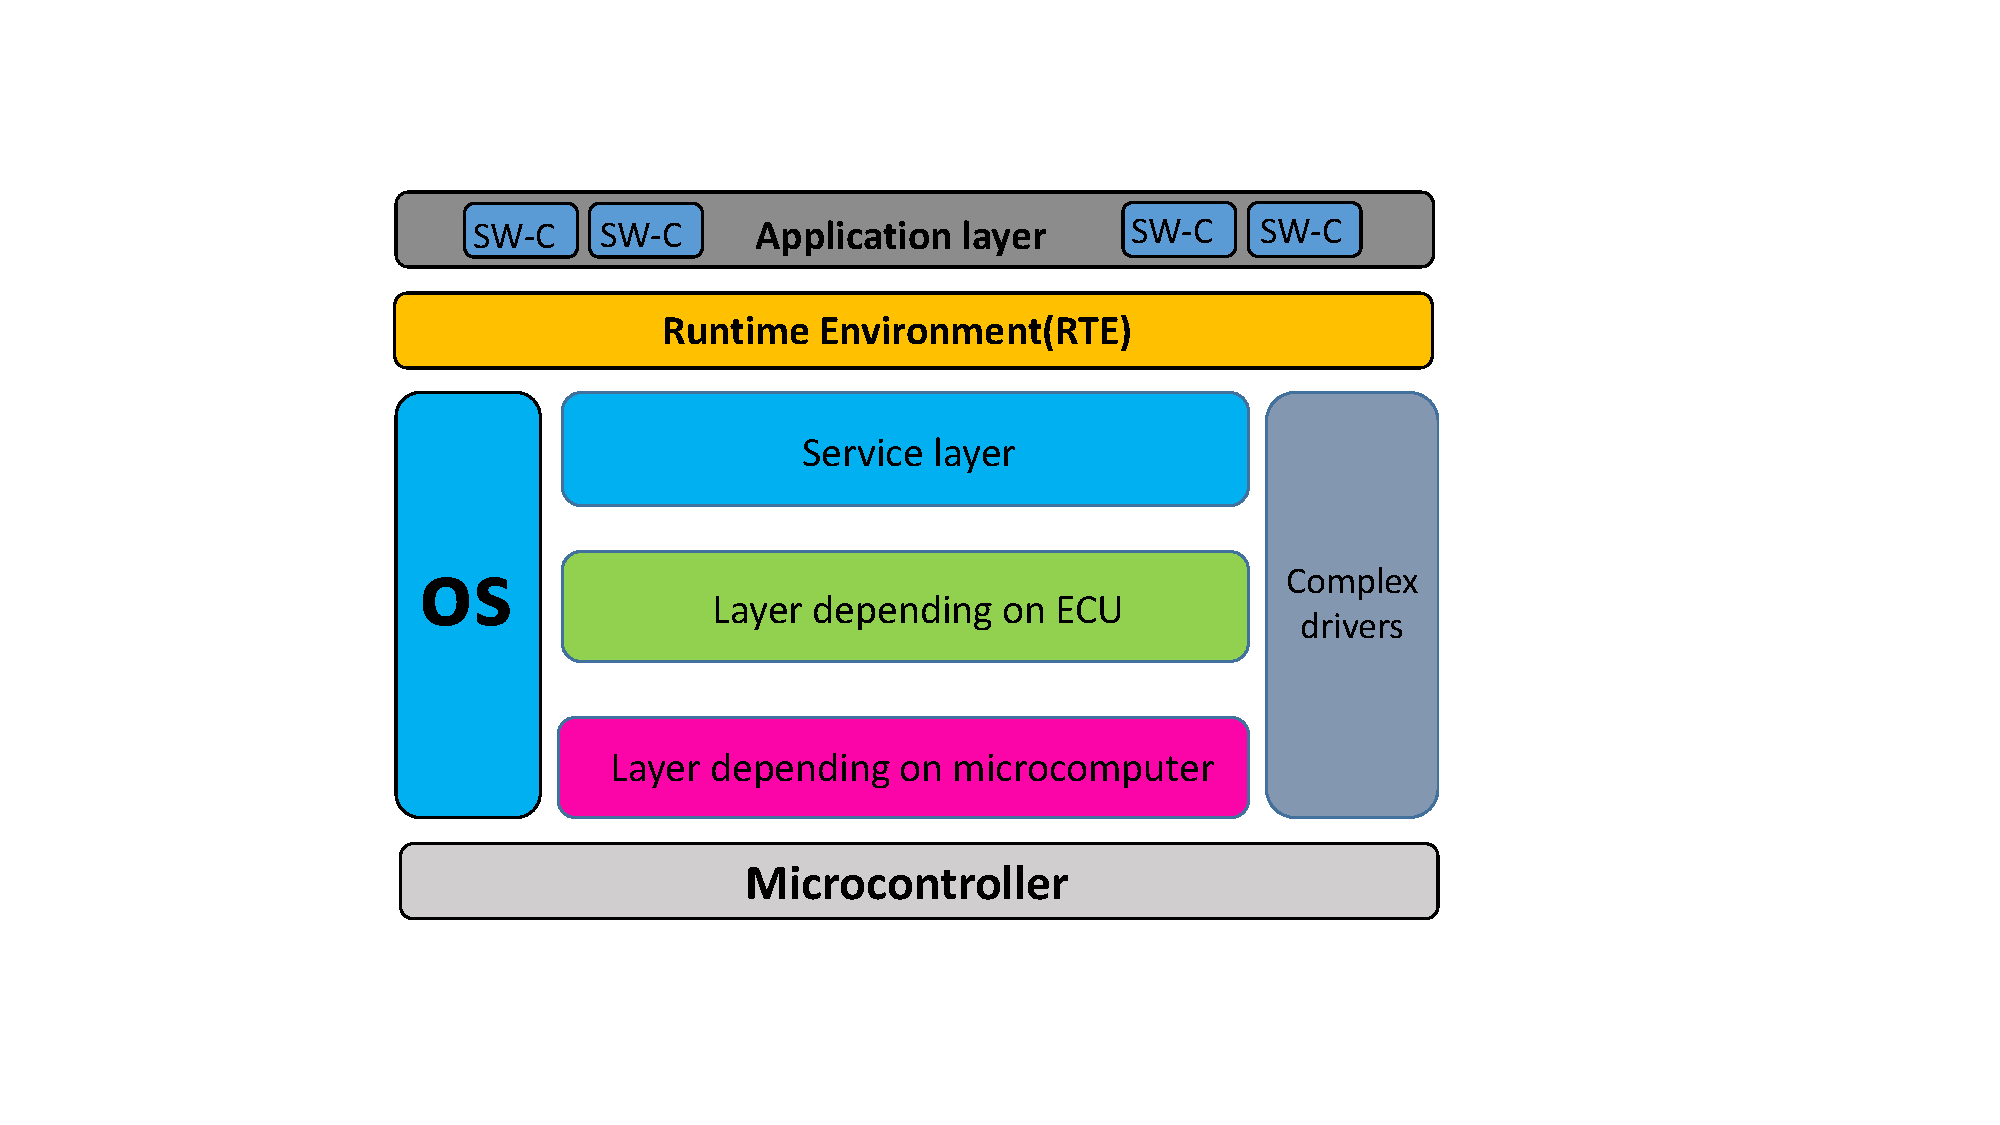
\includegraphics[width=10cm,clip]{figure3.pdf}
	\caption{fig1}
	\label{fig1}
\end{figure}

 {\bf Organization:} The rest of this paper is organized as follows.
Section2 provides a fundamental knowledge for mapping method from block diagrams to runnables.
Section3 gives an existing mapping algorithm and problem of it.
Section4 proposes an extended method algorithm.
Section5 measures and prepare with existing method and new one.
Section6 discusses related work.
Section7 concludes this paper.   
\section {A FUNDAMENTAL KNOWLEADGE}
\subsection{SR model}
An SR model is used for modeling systems, which many things are happening concurrently.
Whereas a dataflow model is good at managing currents of data, a SR model is good at managing sporadic data, where events do not have to exist.
A SR model can detect or adapt faults by that events do not exist.
Therefore, a SR model can implement precise control.
SR model is a model expressed by a synchronous block diagram (SBD).
SBD has a set of subsystems or components S = $\left\{C_j\right\}$. Each Component $C_j$ has blocks 
$B^j = \left\{{{b_1}^j, {b_2}^j,...,{b_{m^j}}^j}\right\}$, a set of inputs $X^j = \left\{{x_1}^j,{x_2}^j,...,{x_{p^j}}^j\right\}$,
and a set of outputs $Y^j = \left\{{x_1}^j,{x_2}^j,...,{x_{p^j}}^j\right\}$.
Each block ${b_i}^j$ has a period and the worst case execution time (WCET) ${\gamma_i}^j$.
Each block is classified as either a combinational or a sequential block.
A combinational block does not have state, so its outputs depend on only its input.
A sequential block has state, and it is classified as either a Moore-sequential or a non-Moore-sequential block \cite{Lublinerman:2009:MCG:1480881.1480893}.
Outputs of Moore-sequential block only depend on state, not inputs.
Therefore, a combinational and  non-Moore-sequential block has execution order constraint.
For each ${b_i}^j$, $Pred({b_i}^j)$ is defined, and is a set of directly connected with input ports of the block.
Similarly, $Succ({b_i}^j)$ is a set of directly connected with output ports of the block.
\begin{figure}
	\centering
	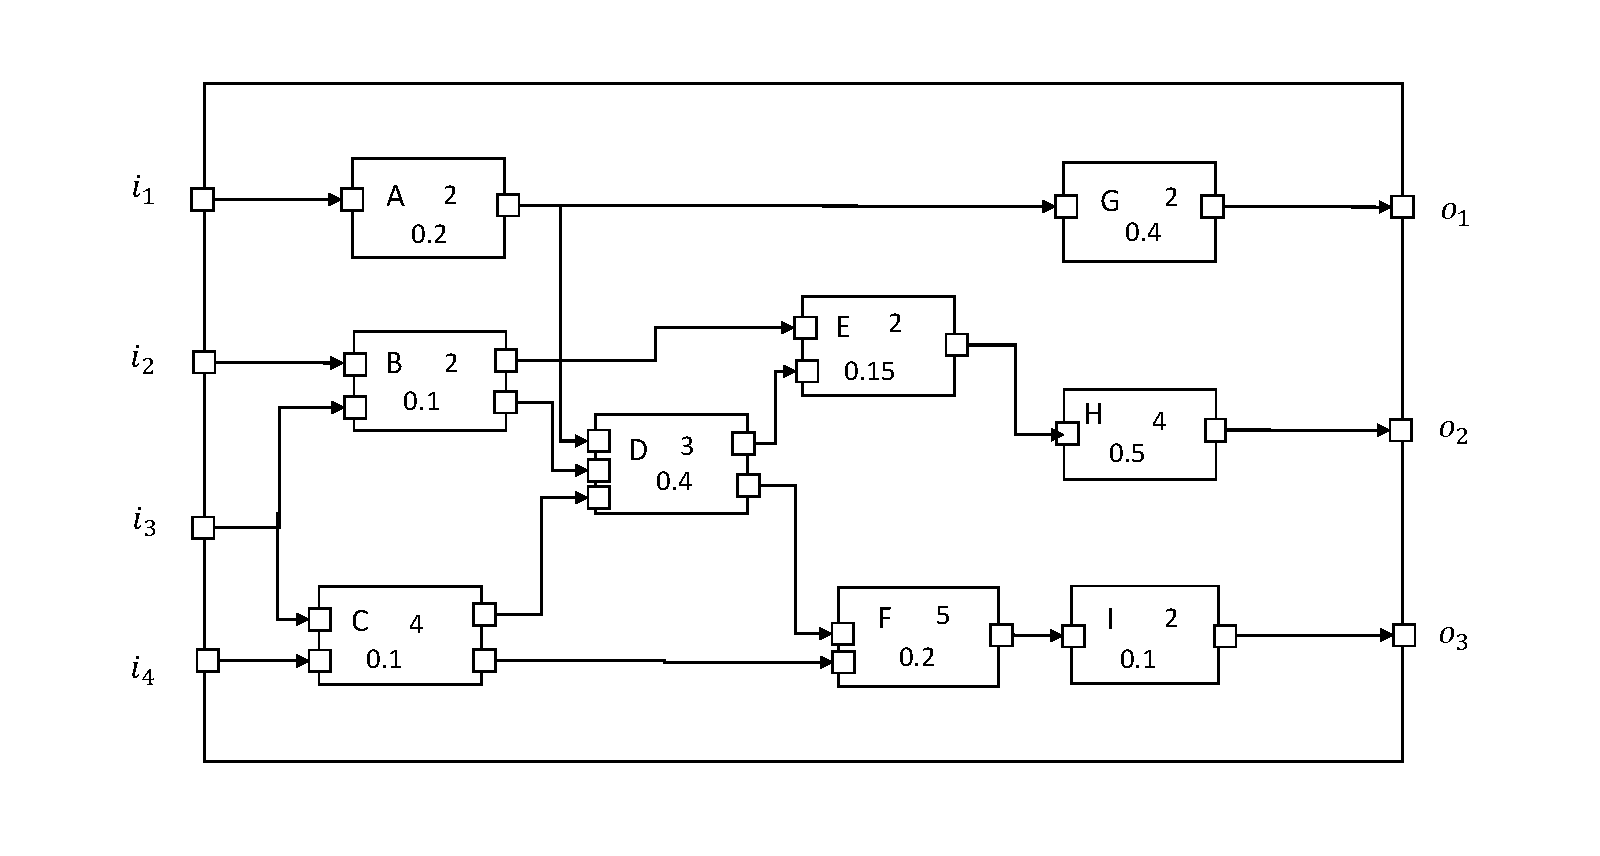
\includegraphics[width=9cm,clip]{figure5.pdf}
	\caption{figure2}
	\label{fig2}
\end{figure}

Figure2 shows an example of SR model with eight blocks labeled A to I, four inputs, and three outputs.
Upper right numeral is period, and lower is the WCET.


\subsection{Firing Timed Automaton}
 Time block diagrams are a kind of diagrams with triggers.
Boolean signal x is called the trigger of a block A when the block A is fired by signal x. 
If x is trigger of block A, A can be fired only when x is true.
(One block can have at most one trigger.)
Time block diagrams have a trigger which is true when it becomes predetermined time.
The trigger like this is called firing time specification (FTS).
There are two notations for FTS.
One notation is called a PPP.
A PPP represents firing time with pair period and phase.(Figure)
The other way is  automaton.
A FTA is an automaton to describe activation events that consist of union of periodic systems.
In other words, a FTA is suitable to define runnable activation events which is periodic.
 A FTA {\it A} is a pair ${\it A} = (\theta,S)$. $\theta$ is a base period, and it is  the time that it takes for transition. 
$S = (V,v_0,F,\delta)$.
$V = {v_0,v_1,...,v_n}$ is a set of vertexes.
$v_0 \in V$ is initial vertex.
$F \subseteq V$ is the subset of firing vertexes.
$\delta : v_{i-1} \rightarrow v_{i}$ is a link or transition.
If $v_n \rightarrow v_0 \in \delta$, the FTA is a cycle.
The cycle period of the FTA is $\Theta = \theta * (n+1)$.
Now, extending FTA, we want to capacitate for describing FTS with automaton.
A runnable is unit of blocks.
Therefore, a runnable has a property similar to blocks.
A runnable $r_k$ has blocks $B^k = \left\{b_1^k,b_2^k,...,b_{n^k}^k\right\}$, period $t_k$, WCET $\gamma_k$.
$Pre(r_k)$ is set of directly $r_k$ depending runnables.
$Suc(r_k)$ is set of directly depended runnables by $r_k$.

\begin{figure}
	\centering
	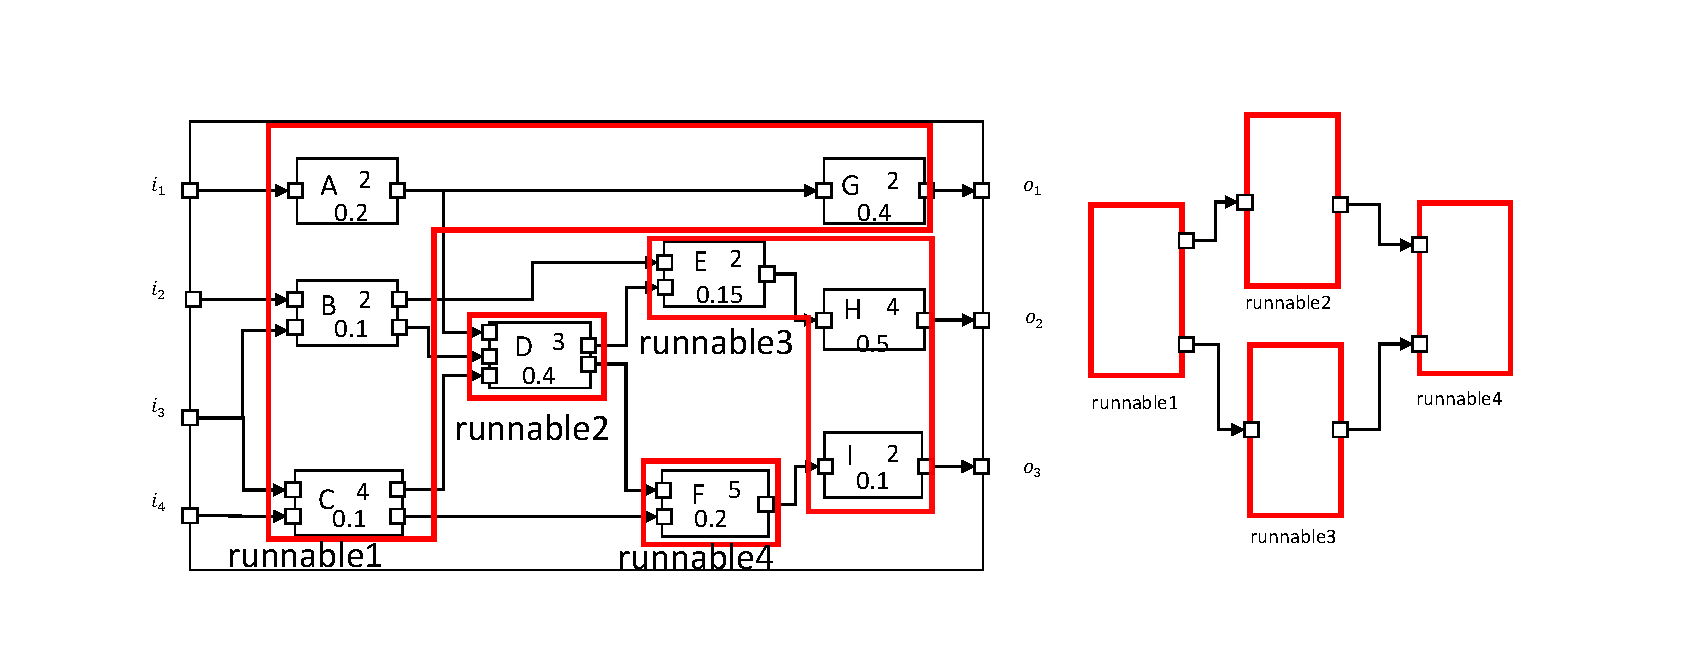
\includegraphics[width=10cm,clip]{figure7.pdf}
	\caption{figure3}
	\label{fig3}
\end{figure}

\begin{figure}
	\centering
	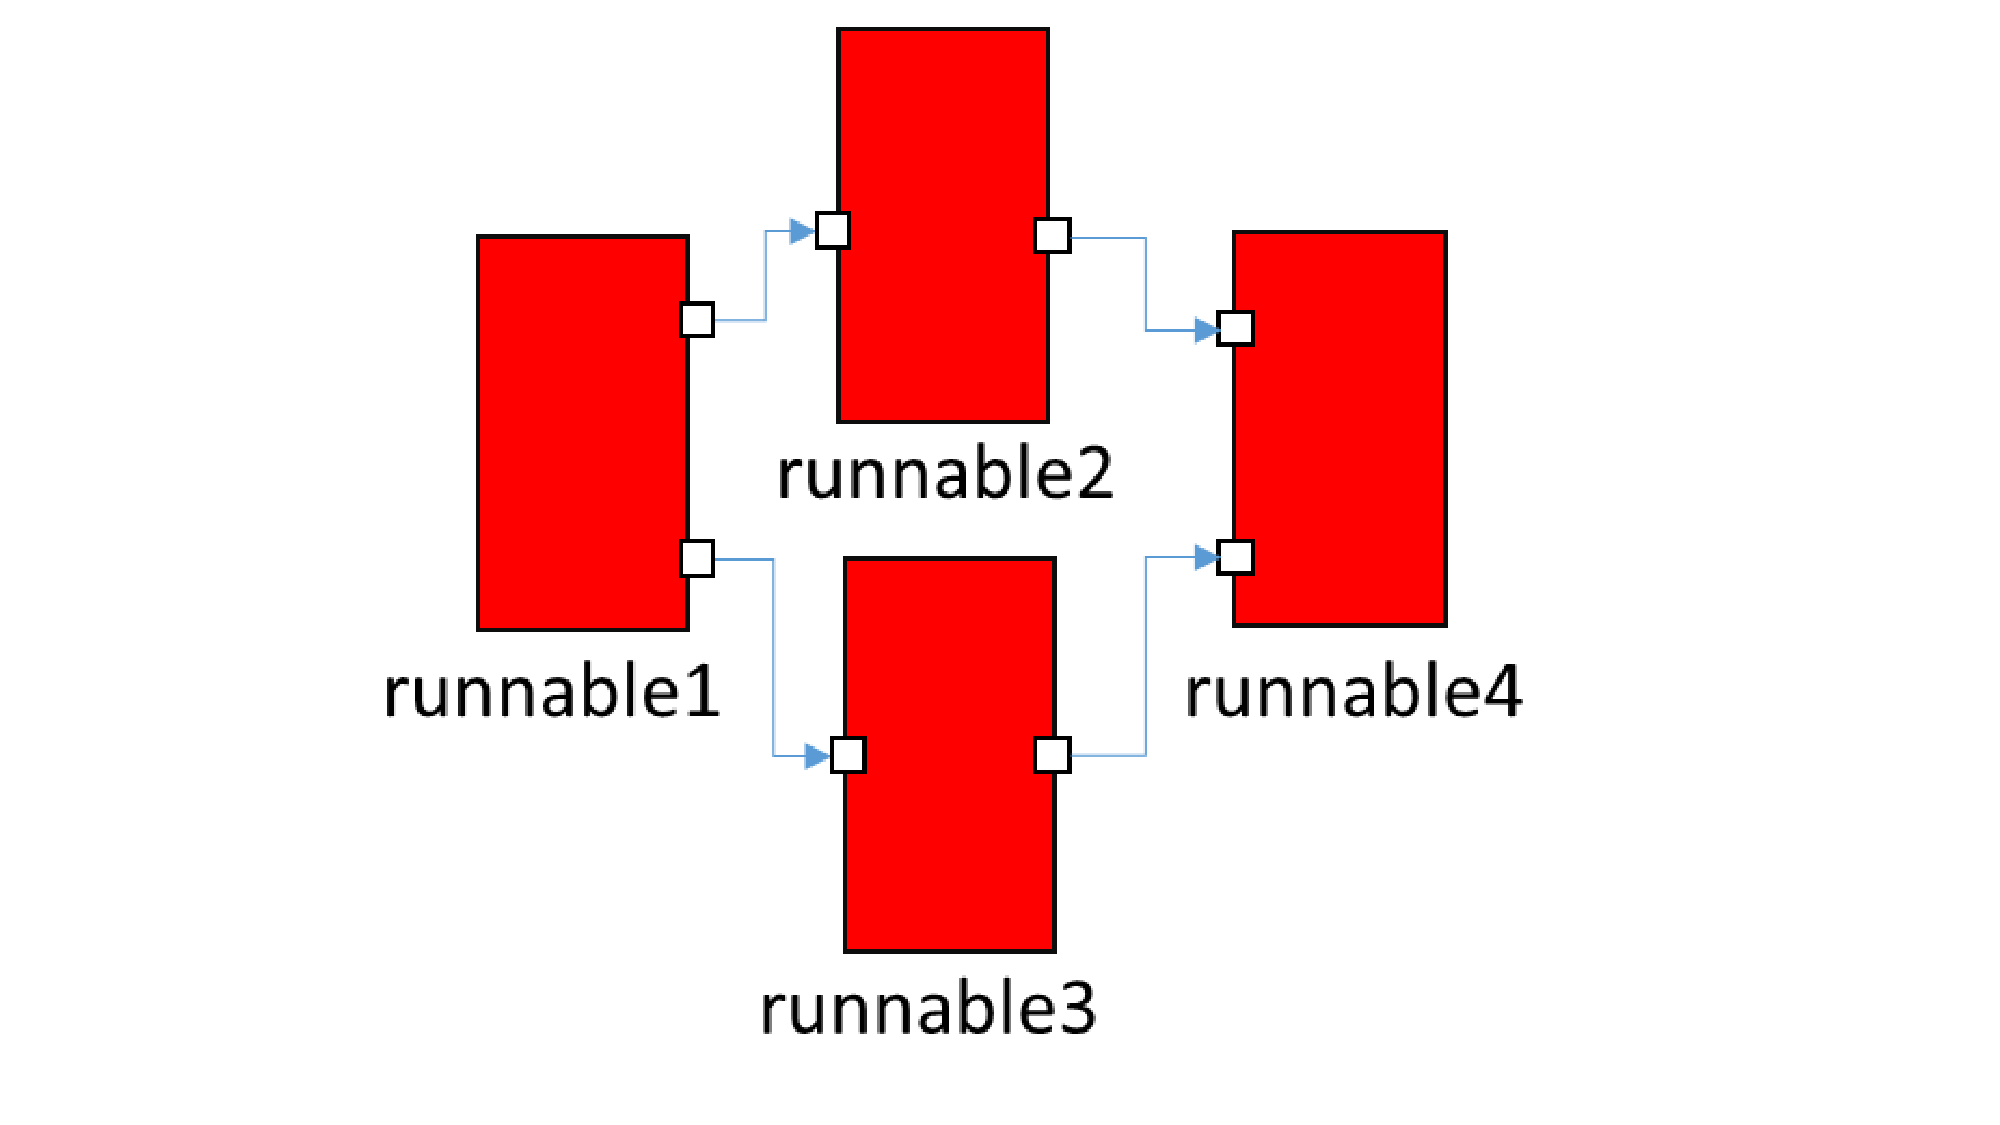
\includegraphics[width=10cm,clip]{figure8.pdf}
	\caption{figure4}
	\label{fig4}
\end{figure}

Figure3 is the example of block mapping from SR model to runnables.
Figure shows dependency of resulting runnables.
Now, I would like to express  the runnable1($r_1$) of Figure3 in FTA.
$B_1 = \left\{block A, block B, block C, block G\right\}$.
In the case that base period is one, FTA is shown upper in the Figure5.
By the way, greatest common divisor(GCD) of each blocks in $B_1$ is two.
Therefore, the base period of FTA $\theta$ is changed to two .
Actually, only when it is a multiple of GCD, blocks fires.
When base period is one, the runnable fires all the time, but if we can change base period to GCD, the runnable firing frequency decreases, and the runnable will fire if and only if some of its blocks need to fire. 
 Once the FTS of runnable is updated, blocks of the runnables must be updated.
A period of blocks of the runnable changes period divided by new runnable period, which period of block A, B, C, G are 2/2, 2/2, 4/2, 2/2 respectively.
Therefore, FTA of the runnable become below in Figure5.  
 WCET is sum of each blocks in $B_1$,and $gamma_1$ is 0.8.


\begin{figure}
	\centering
	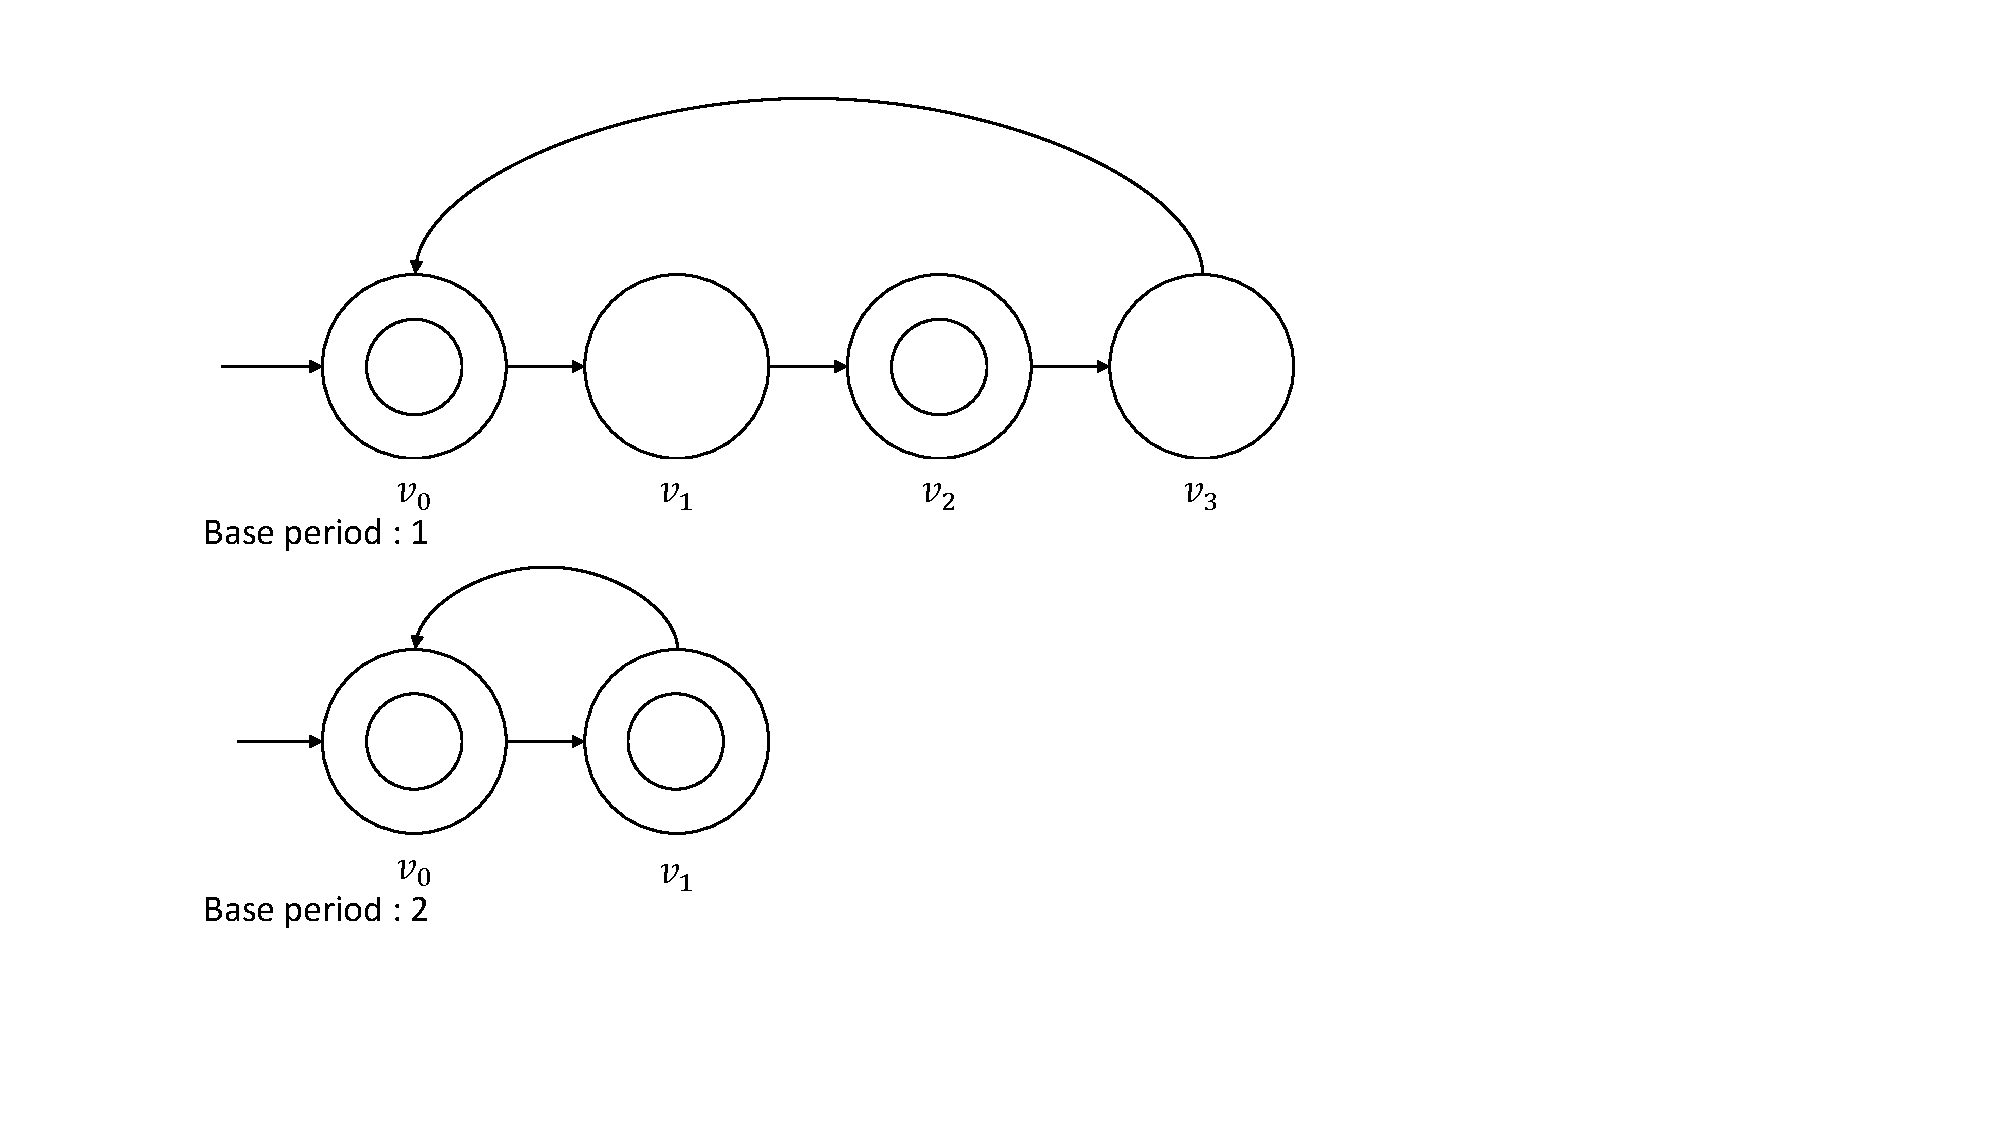
\includegraphics[width=10cm,clip]{figure9.pdf}
	\caption{figure5}
	\label{fig5}
\end{figure}


\subsection{Cycle dependency}
 Cycle dependency is that exist cycle in execution order constraints. <See the Figure>
\begin{figure}
	\centering
	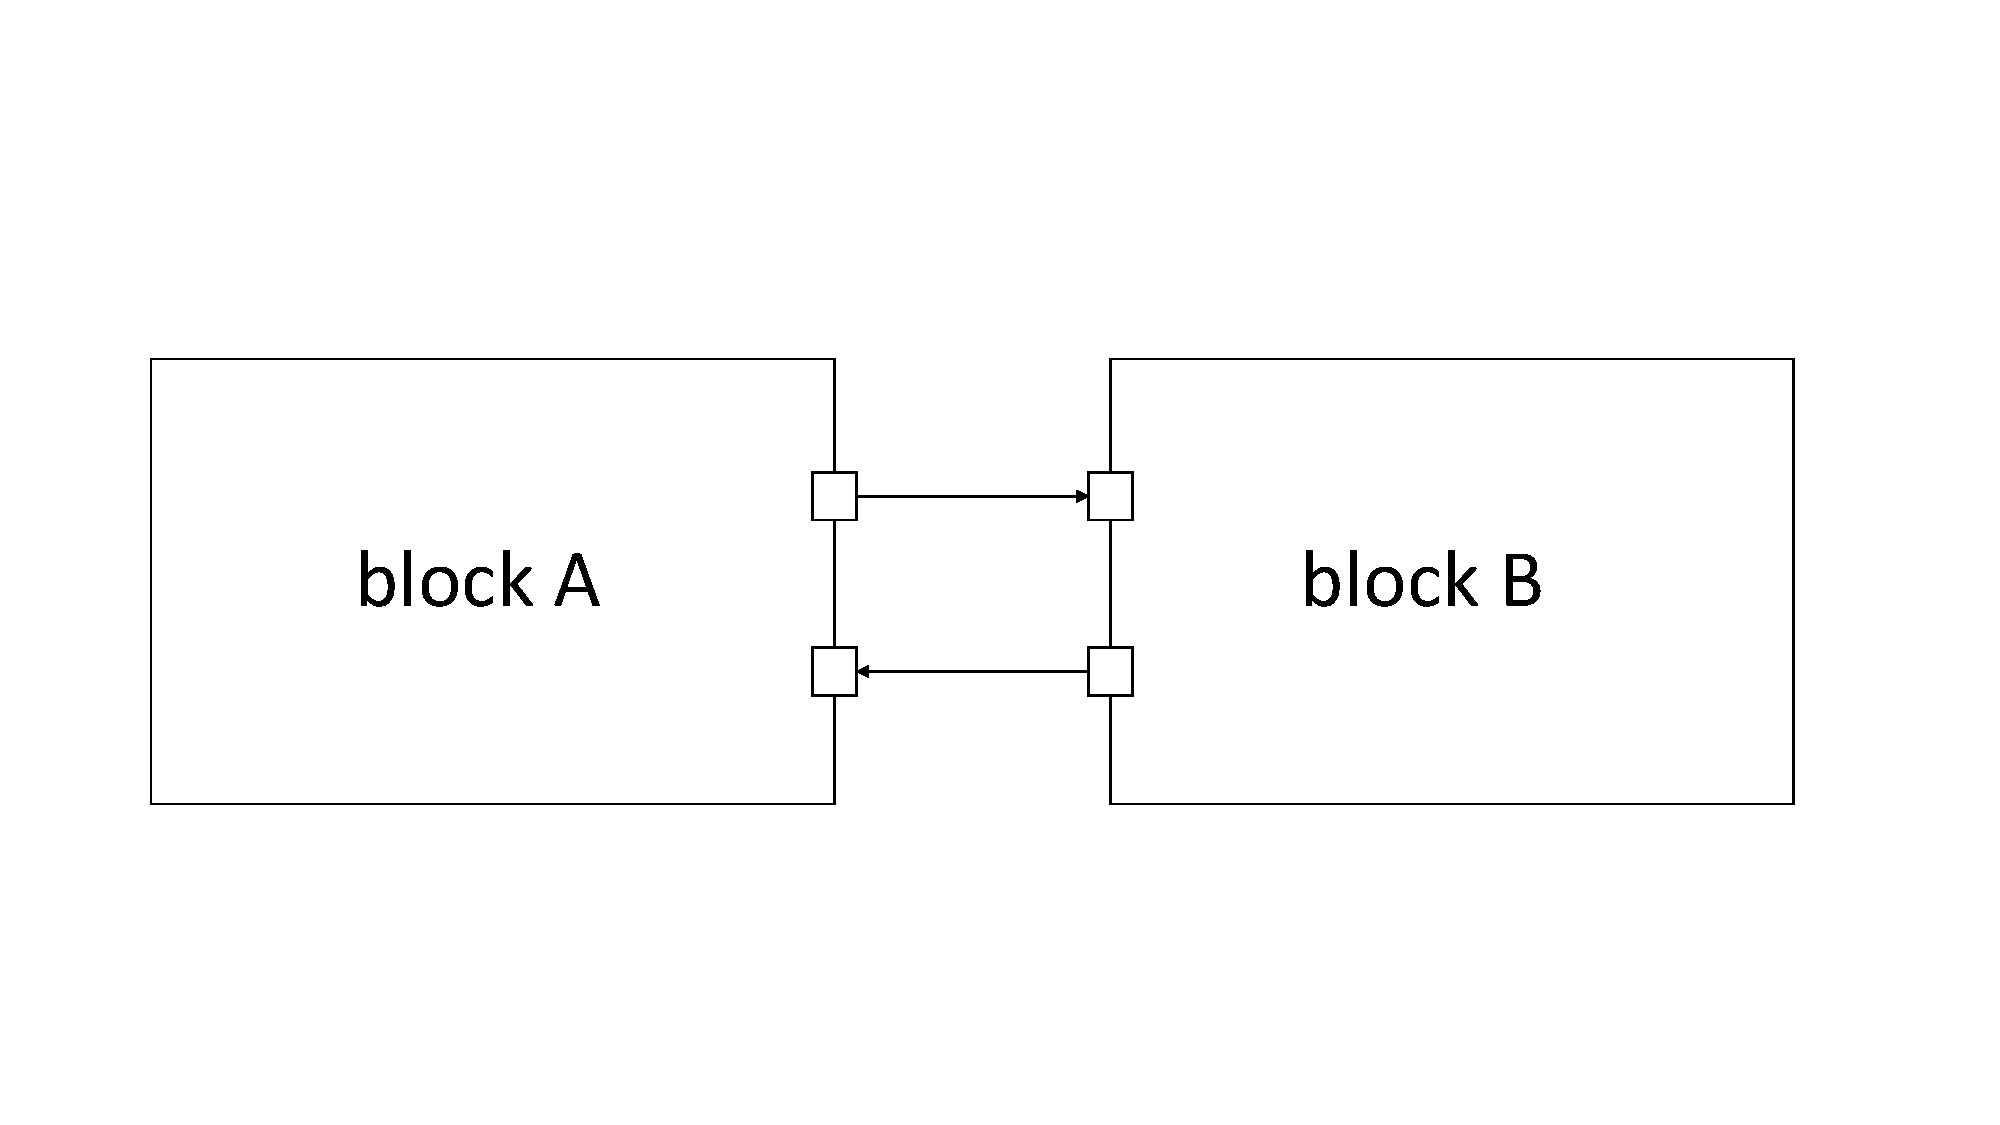
\includegraphics[width=10cm,clip]{figure4.pdf}
	\caption{figure6}
	\label{fig6}
\end{figure}
 Figure4 shows an example of cycle dependency.
The output of block A depends the output of block B, but the output of block B also depends on output of block A.
Because of this, both outputs is not able to be calculated.
When a block diagram has a cycle dependency, some blocks which compose cycle dependency are Moore-sequential, all output must be able to be calculated.
\subsection{Three metrics}
 In mapping from blocks to runnables, there are three evaluation criterias in below.
\subsubsection{Modulality}
 Modulality is measured by the number of generated runnables.
The smaller the number is, the higher the degree of modulality is.
Runnables hide the internal imformation, so when the degree of modulality is very high, that is, the number of runnables is considerably small compared with the number of blocks,
the internal structure become difficult to grasp it.
\subsubsection{Reusability}
 Reusability of generated runnable is measured whether it dose not have any false input-output dependencies.
\begin{figure}
	\centering
	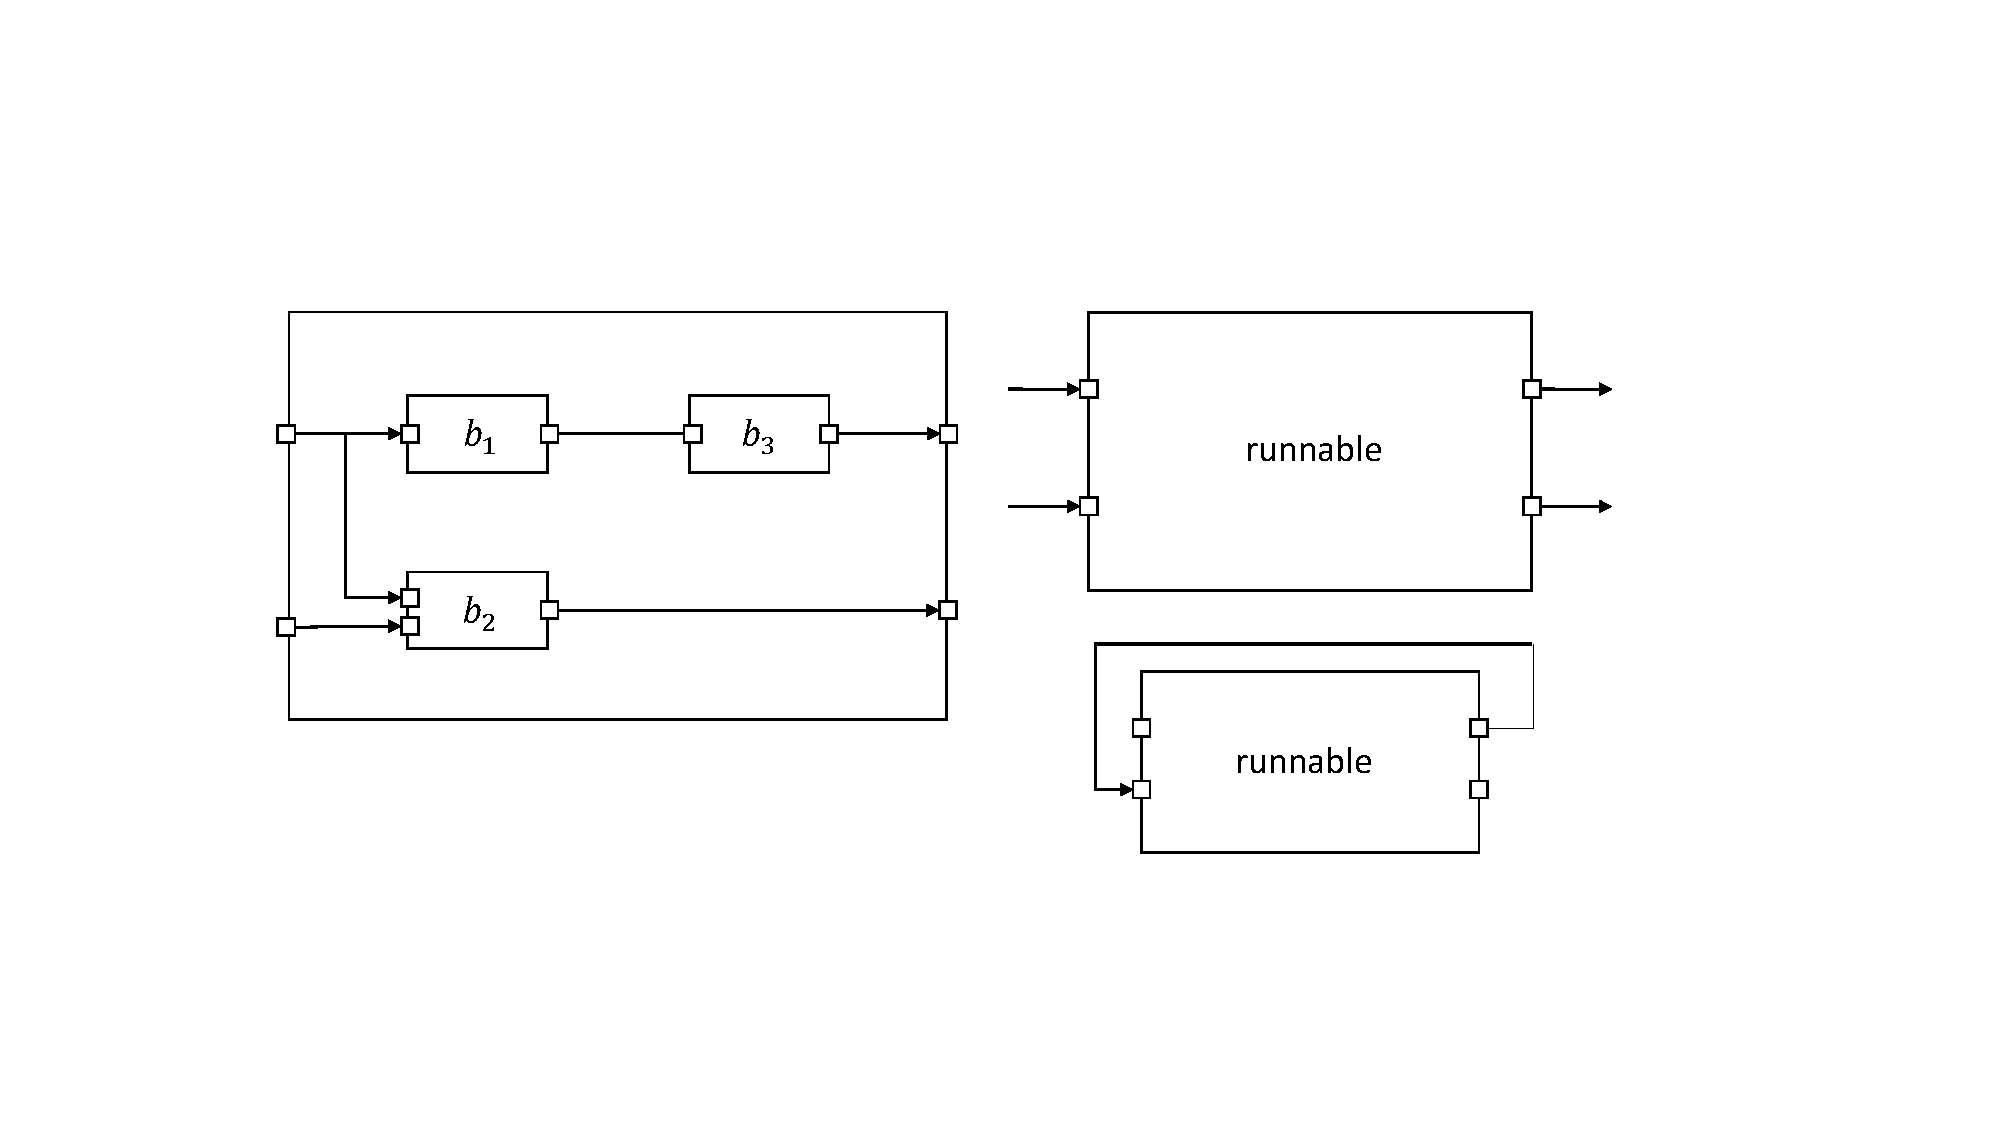
\includegraphics[width=10cm,clip]{figure6.pdf}
	\caption{figure7}
	\label{fig7}
\end{figure}
 The component of left side of Figure2 consists of three blocks, two inputs, and two outputs.
Now, let this component map one runnable. (right side of Figure2)
Because runnable makes internal information black box, $o_1$ and $o_2$ depend on $i_1$ and $i_2$ from external imfomation.
In the other word, the link like Figure2 is refused.
However, in practice $o_1$ does not depend $i_2$, and the feedback link is safe. 
In this way, qualitatively when the number of runnable is as many as the number of blocks, false dependencies are difficult to exsist.
Modulality and Reusability are trade-off relationship.
\subsubsection{Schedulability}
 Schedulability expresses index of whether the generated runnables are able to schedule.
If generated runnables have scheduling bottlenecks, it becomes low.
Scedulability is meansured as follows.
 Local utilization $u_i = c_{i0} / \rho_i$ is defined for each vertexes $v_i$ in  FETA of its runnable.
$c_{i0}$ is unconditional WCET of $v_i$, and $\rho_i$ is defined as $\rho_i = \theta_k * d_i$.
$\theta_k$ is the period of runnable  $\gamma_k$, and $d_i$ is destance of FETA path from $v_i$ to the next firing vertex.
$R$ is the set of runnable for a component $C$.
For each runnable $\gamma_k$, let the maximum local utilization  be $u_{k}^{max}$, where $u_k^{max}$ is the most among $u_i$ in $\gamma_k$.  
But, let $c_{i0}$ of not firing nodes be 0.
The sum of maximum local utilization of each runnables is denoted as $U_l$.
$U_l$ is able to be computed as:
\begin{equation}
 U_l = \sum_{r_k \in R} u_{k}^{max}\;where\;u_{k}^{max} = \max_{v}(u_{k}^{v})
\end{equation}

The component utilization $U_c$ is computed as:
\begin{equation}
U_c = \sum_{b_i \in C} \frac{C_i}{T_i}
\end{equation}
where $C_i$ is WCET of $b_i$ and $T_i$ is period of $b_i$.
 Alfa ratio $\alpha = U_l/U_c$ is defined.
When we compose runnable from a component, we can compute alfa, and schedulability can be measured by alfa.
There is following theorem in alfa.
Theorem The alfa ratio $\alpha_u = \frac{U_l}{U_c}$ for any runnable implementation R is greater than or equal to 1, i.e. $U_l \le U_c$.
The ratio is 1 if and only if the blocks with the same period are grouped in the same runnable.

\begin{figure}
	\centering
	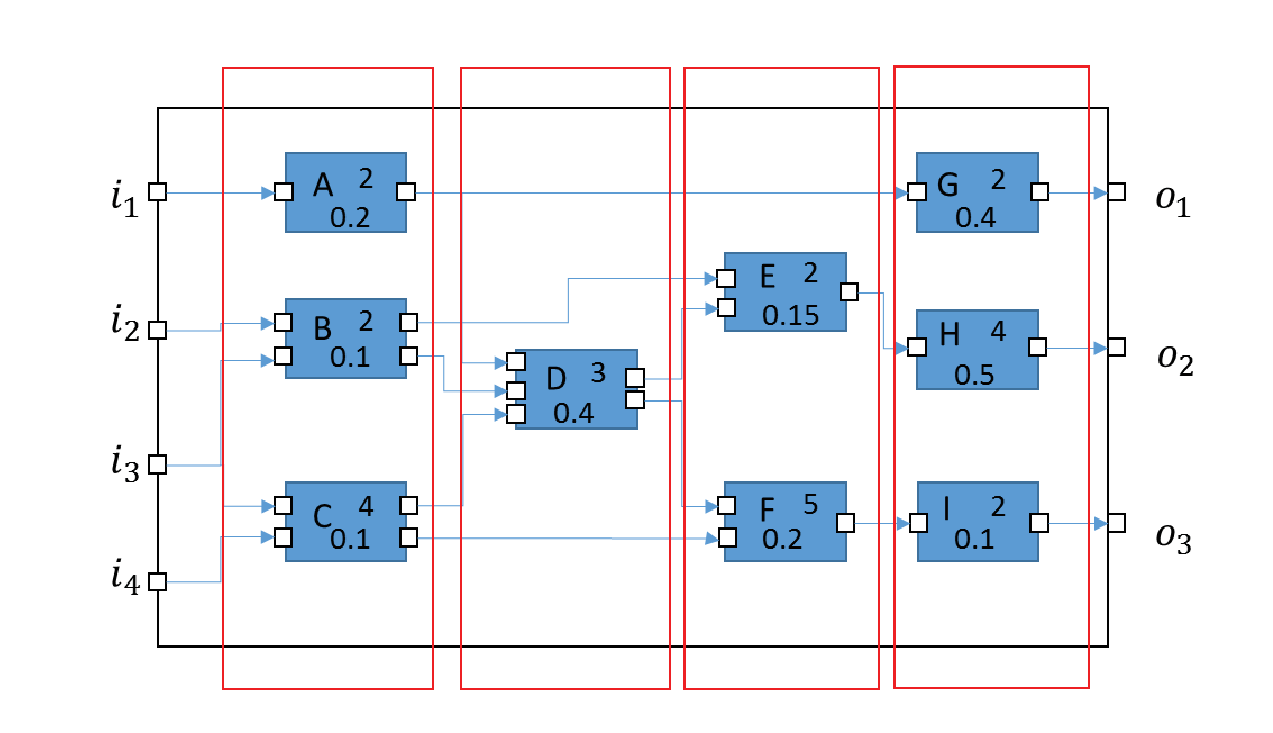
\includegraphics[width=10cm,clip]{figure1.eps}
	\caption{figure8}
	\label{fig8}
\end{figure}


\begin{figure}
	\centering
	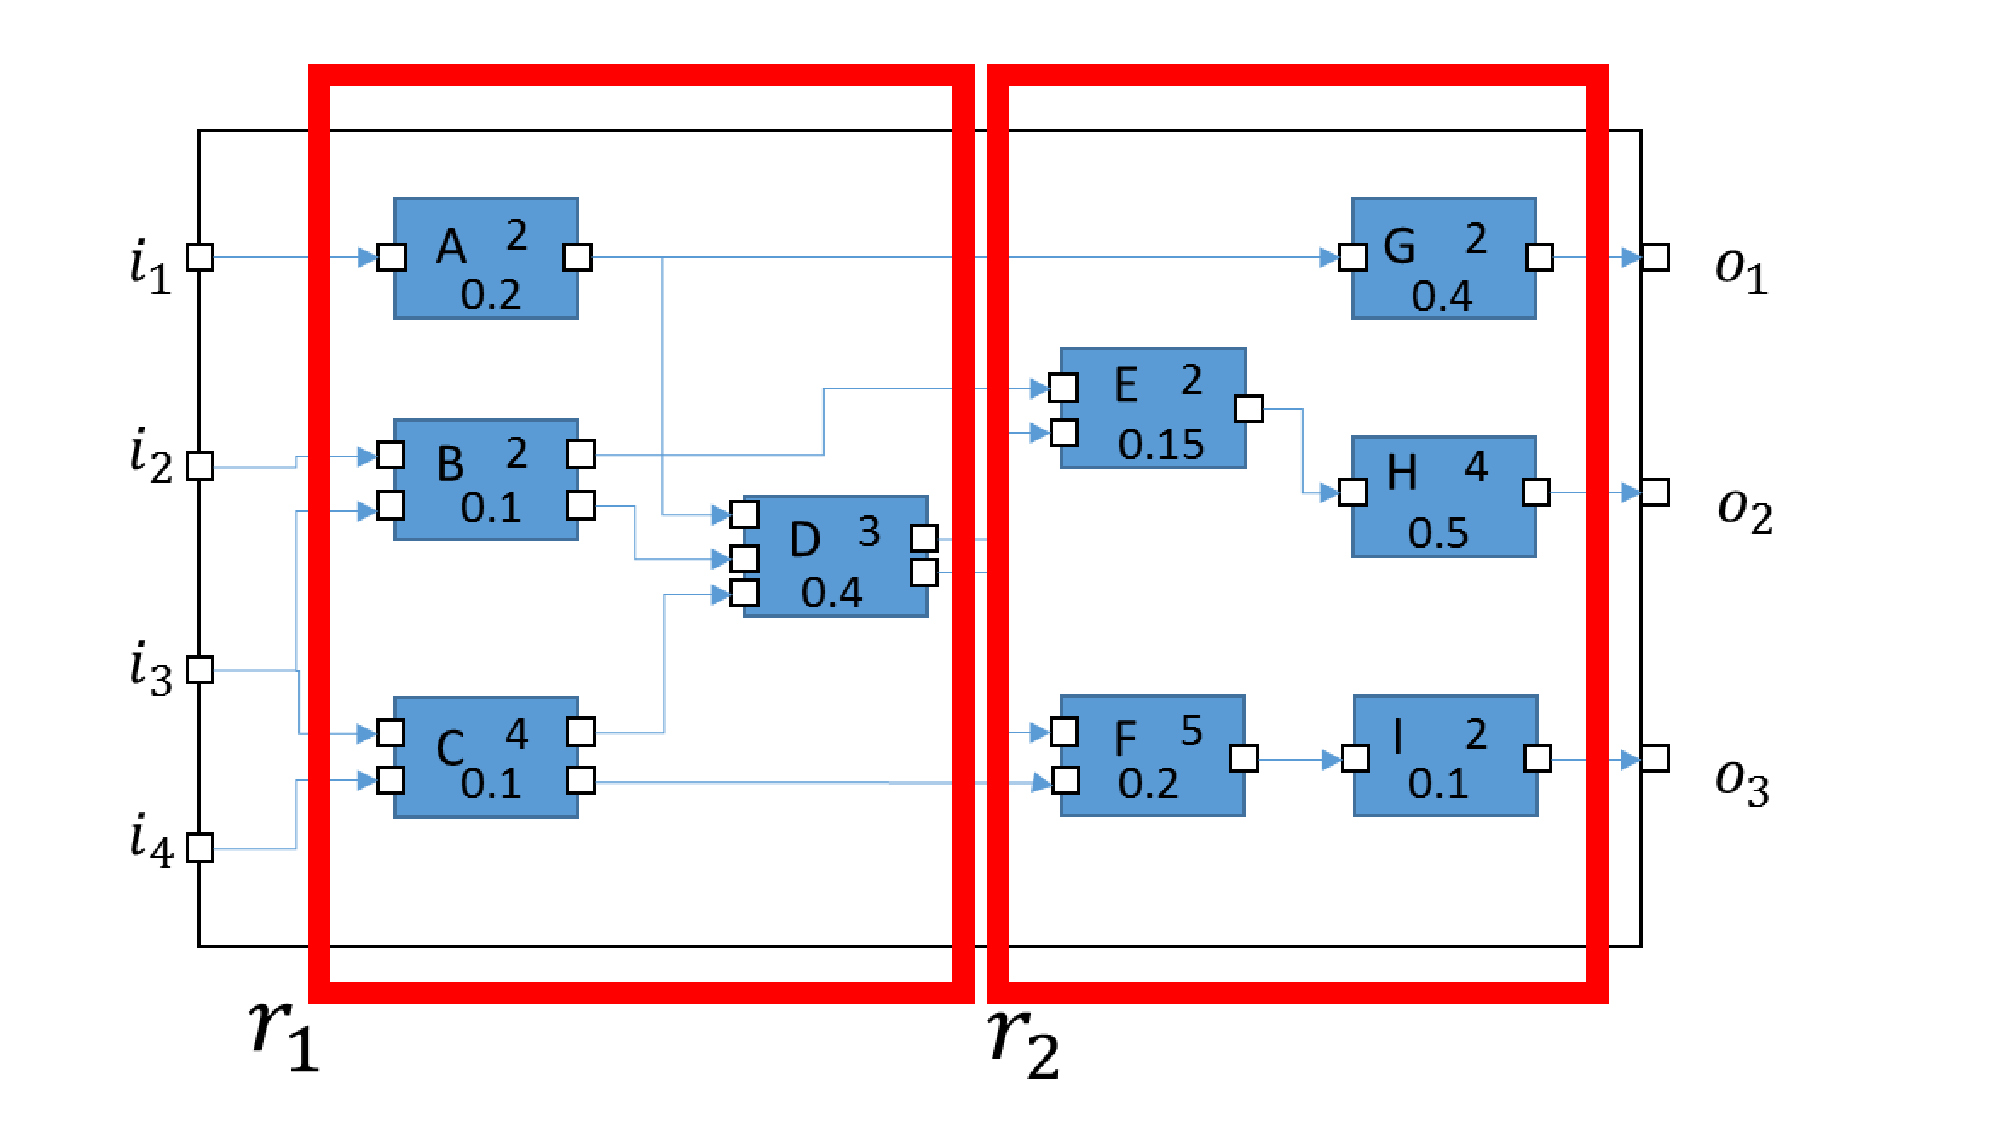
\includegraphics[width=10cm,clip]{figure2.pdf}
	\caption{figure1}
	\label{fig9}
\end{figure}


\section{TOP-DOWN METHOD}
 A top-down method is proposed in \cite{Deng:2015:MSF:2735960.2735972}.
The top-down method is one of runnable synthesis algorithms to trade off schedulability and modularity while achieving maximum reusability and minimum code size, using FTA and alpha ratio. 
First step is to find a runnable generation that optimizes modularity, while achieves maximum reusability with a MILP formulation.
Next step is to decompose the runnables to improve schedulability until obtaining desire alfa ratio and the number of runnables.
During this process, maximum reusability and minimum code size are preserved, because decomposing runnables does not make false dependency.
 The initial MILP formulation is as follows.
The important purpose of this step is obtaining the runnable generation with no false dependency.
Maximum reusability is preserved if it is satisfied with constraints with respect to relationships among inputs and outputs.
X and Y denote the set of input and output virtual block.
B denotes the set of original blocks.
An input and output block must be mapped to the same runnable as the block that the input or output belongs.
$C_{b_i}$ denotes the component that $b_i$ belongs.
Similarly, $C_{r_m}$ denotes the component that $r_m$ belongs.
$g_{b_i,r_m}$ is a binary value, which is one if $b_i$ is mapped to $r_m$, otherwise zero.
A binary value $h_{r_m,r_n}$ denotes a relationship between runnables, and $r_m$ must be implemented before $r_n$ when it is one.
$Q_{b_i,b_j}$ preserve a relationship between blocks and is computed by using Breath-first search (BFS).
BFS is used before the MILP formulation.
$Z_{r_m}$ denotes whether there exists at least a block that is mapped to $r_m$, is bynaly value.
Therefore, $\sum_m Z_{r_m}$ is a number of runnables.
(3) is the objective formulation, it optimizes modularity.
(4) must be satisfied by definition of $Z_{r_m}$ and $g_{b_i,r_m}$
(5-8) is the constraints on mapping from blocks to runnables.
The constraints (9-11) denotes definition of the causality relationship among runnables.
(12) is condition not to make any false input-output dependencies. 

\begin{eqnarray}
 min \sum_{m} Z_{r_m} \\
 Z_{r_m} \geq g_{b_i,r_m} \forall b_i,r_m \in B,R \\
 \sum_m g_{b_i,r_m} = 1 \forall b_i,r_m \in B,R \\
 g_{b_i,r_m} = 0 \forall C_{b_i} \neq C_{r_m} \\
 g_{b_i,r_m} = 1 \forall b_i,r_m \in X,Y \wedge m = i \\
 g_{b_i,r_m} = 0 \forall b_i,r_m \in X,Y \wedge m \neq i \\
 h_{r_m,r_n} \geq h_{b_i,r_m} + g_{b_j,r_n} + Q_{b_i,b_j} - 2 \\
 h_{r_m,r_n} \geq h_{r_m,r_l} + h_{r_l,r_n} - 1 \\
 h_{r_m,r_n} + h_{r_n,r_m} \leq 1 \\
 h_{r_m,r_n} = Q_{b_m,b_n} \forall b_m,r_m \in X \wedge b_n,r_n \in Y
\end{eqnarray}

 However, a computational complexity of the MILP formulation is high.
Therefore, by using the below method, we can get alternative solution for modularity optimization.   

\begin{algorithm}
\caption{modularity optimization solution to fill in for the MILP formulation}         
\label{alg1}                          
\begin{algorithmic}[1]
\STATE Let each block $b_i$ in S be initially mapped to each task $\gamma_i$.
\STATE Let $\Gamma = {\gamma_i}$, and change = true.
\WHILE {change}
	\WHILE {$\exists b_i \in G_k, b_i \in G_k, s.t. Pred(b_j)$ and there exists no input directly connected to $b_j$}
		\IF {schedulable\_after\_merge($b_i,b_j$)}
			\STATE merge\_blocks(b\_i,b\_j); merge\_task($\gamma_i,\gamma_j$).
		\ENDIF
	\ENDWHILE
	\WHILE {$\exists b_i \in G_k, b_i \in G_k, s.t. Succ(b_j)$ and there exists no output directly connected to $b_i$}
		\IF {schedulable\_after\_merge($b_i,b_j)$}
			\STATE merge\_blocks($b_i,b_j$); merge\_task($\gamma_i,\gamma_j$).
		\ENDIF
	\ENDWHILE
	\STATE change = false
	\IF {$\exists b_i \in G_k, b_i \in G_k, s.t.$ max\_reusability\_after\_merge($b_i,b_j$) and schedulable\_after\_merge($b_i,b_j$)}
		\STATE merge\_blocks($b_i,b_j$); merge\_task($\gamma_i,\gamma_j$); change = true.
	\ENDIF
\ENDWHILE
\RETURN $\Gamma$
\end{algorithmic}
\end{algorithm}

 This alternative heuristic acheives solution quickly, but this solution is not optimal.
Therefore, if you want to get optimal modulality solution of smoal systems, you should use the MILP formulation.


Next, Algorithm 2 decomposes obtained runnable generation to improve schedulability.
The algorithm finds runnable $r_m$ that has most maximum local utilization among runnables, and decomposes $r_m$ to $r_n$.
The algorithm sorts blocks of $r_m$ in period descending order.
It tries to decompose each block in order, and if there are no cycle dependencies, the block is decomposed, and mapped to $r_n$.
Once it finds block that can be mapped to $r_n$, a variable found becomes true, and period $T_n$ of $r_n$ become the period of the block mapped.
If found is true, candidate blocks mapped to $r_n$ are blocks that has the same period as $T_n$.
At the end, alpha ratio is computed, and N is added 1 to.
This continues until obtaining desire alpha ratio or target $\acute{N}$.


\begin{algorithm}                      
\caption{Top-down method}         
\label{alg2}                        
  
\begin{algorithmic}[1]
\STATE In First step, we obtain a runnable generation p that is optimal modularity, while it introduces no false dependencies, using the MILP formulation.
\STATE In Second step, we improve schedulability as below until we obtain desire alfa ratio and target number of runnables.
\STATE $\alpha_u$ = ComputeAlpha()
\WHILE {$\alpha_u > \acute{\alpha_u} \vee N < \acute{N}$}
	\STATE Let $r_m$ be the runnable with maximum $u{_m}^{max}$ among those that have different period blocks.
	\STATE For each $b_i \in r_m$, order $b_i$ based on descending $T_{b_i}$
	\STATE $r_n = \phi$, found = false, $T_n = 0$
	\FOR {$b_i \in r_m$ in order}
		\IF {found = false}
			\STATE $r_n = r_n \cup b_i$
			\STATE $p_t = $ decompose($r_m,r_n$)
			\IF {existsCycle($p_t$)} 
				\STATE $r_n = r_n - b_i$
			\ELSE 
			\STATE $p_b = p_t$, found = true, $T_n = T_{b_i}$
			\ENDIF
		\ELSE
			\IF {$T_{b_i} = T_n$}
				\STATE $r_n = r_n \cup b_i$
				\STATE $p_t = decompose(r_m,r_n)$
			\ELSE
				\STATE $p_b = p_t$
			\ENDIF
		\ENDIF
	\ENDFOR
	\STATE $p = p_b, \alpha_u = ComputeAlpha(), N = N + 1$
\ENDWHILE
\end{algorithmic}
\end{algorithm}

 This sequential of method has some problems.
First, we discuss the heuristic algorizm that make the initial set of runnables.
Maiking the set of runnables, the heuristic must satisfy constraints that the set of runnables has no false dependency and do not introduces false dependency as a result of {\it decompose()}.
Because of this, the heuristic executes many runnables, that is, it is low modulality.

Next, we examine the top-down method.
This method uses the set of runnables gotten by the heuristic, and finds the solution with {\it decompose()}.
{\it decompose()} can decompose a runnable if the the set of runnables including the result runnable does not have cycle dependency.
The decomposed runnable is determined according to the maximum local utilization, and the decomposed block is selected depending on maximum vertex utilization.
At this time, if the block is not seccessed at be decomposed due to cycle dependency, more effective decomposing can not be implemented.
If the block is not able to be decomposed in succession, total utilizatin $\alpha$ is not much improved.
This becomes the bottle neck, the number of runnables increases as result.

\section{EXTENDED MAPPING METHOD}
 For resolving the above problems, this section proposes the extended mapping algorizm.
As above, it is a problem that the number of initial runnables is large.
First step, the method obtains an appropriate runnables, which the number of it is the same to the number of outputs of its component.
Note that each block is mapped only one runnable for minimizing code size.
Due to this initial mapping, the number of runnables will decrease compared with existing method, but the generated runnables may introduce false dependency.
Accordingly, extended {\it decompose()} can decompose a runnable if the generated set of runnables do not have false dependency.

The algorithm is as below.


\section{RERATED WORK}
 This section discusses related work with respect to a model based development.

 In multitask software implemeentation of SBDs, blocks to task mapping method is commonly proposed.
In \cite{6871195}, as evaluation objects, timing metrics is proposed, in addition to modulality, reusability, and code size.
Moreover, a new mapping method (TRCM and MRCT) is proposed, considering optimal timing metrics and modulality, while achieving maximum reusability and minimum code size. 

 Automatical code generation is focused on.
In notation FTS of blocks in SBD, all blocks are fired all the time in previous. 
\cite{4550788} discusses triggered and timed block diagrams, and propose FTA that is useful for describing firing time of a unit of snchronous system.
Due to FTA, it become possible to express derails of firing time, block should fire only in designated time.

 Block diagrams are a usuful graphical notation. 
It is used in commercial products such as Simulink and SCADE \cite{Lublinerman:2009:MCG:1480881.1480893}.
With SAT solver \cite{Lublinerman:2009:MCG:1480881.1480893}, code generation that optimizes modularity while maintaining maximum reusability and minimum code size is proposed.

 Robotic middlewares, such as Orocos-RTT \cite{}, is platform that executes component-based applications and abstract functionality, but are difficult to be integrated in a model-based flow with automatic code generation.
 Control applications are designed by synchronous models (Simulink), but the code generated is executed only by a single core.



\section{test}

As shown in \cite{Deng:2015:MSF:2735960.2735972}.
As shown in \cite{6871195}
As shown in \cite{4550788}

As shown in \cite{Lublinerman:2009:MCG:1480881.1480893}
As shown in \cite{Ptolemaeus:14:SystemDesign}

%Refference
\bibliography{ref}

\end{document}
